%\documentclass[twocolumn]{article}
\documentclass[./chem_exercises.tex]{subfiles}
\begin{document}

%\begin{titlepage}
%\maketitle
%\end{titlepage}


%\layout

%\chapter{Syntes av Koppar(II)sulfat}
\textit{\textbf{Tentamen Kemiska beräkningar, 2021-10-27}}
\begin{enumerate}
\item a. Hur definieras kemisk Jämvikt? Motivera!\\
En kemisk jämvikt inträffar i en reversibel reaktion, exempelvis
\begin{flalign*}
\ch{HAc} + \ch{H20}\ch{<=>} \ch{H^+} + \ch{Ac^-}
\end{flalign*}
Ättiksyran löst i vatten bryts upp (joniseras) i acetatjoner och protoner som rekombinerar
till ättiksyremolekyler som i sin tur bryts upp i acetatjoner och protoner.
Till slut blir joniseringstakten och rekombinations takten lika och ingen nettoändring
kan detekteras trots att aktivitet jonisering och rekombination hela tiden pågår på den molekylära
nivån och då har kemisk jämvikt nåtts.
De två olika hastigheterna för jonisering och rekombination behöver inte vara samma utan jämvikten
uppstår därför att rekombination kan bara ske i den mån jonisering skett och återjonisering sker bara
i mån av att rekombination har skett. Detta beskrivs av en ``predator -prey'' typ kopplad differential ekvation
av första ordningen.\\

b. Vad är en bra pH-buffert? Motivera utifrån hur en bra pH-buffert definieras.\\
En pH-buffert är en lösning av en svag syra och dess konjugerade bas tillsatt såsom ett salt
eller en lösning av en svag bas och dess konjugerade syra tillsatt såsom ett salt.
En bra pH-buffert har förmågan att motstå ändringar i pH-värde för små tillsatser av syror eller baser dvs. pH-värdet
hålls konstant.\\

\item Ett nytt lovande läkemedelsämne har tagits fram med kodnamnet YXZ och det har bestämts
genom masspektrometri att föreningen har följande procentuella grundämne sammansättning:
44,2\% kol, 2,48 \% väte, 43,5\% klor och resten syre. Molmassan är cirka 650 g/mol. Bestäm
molekylformeln för ämnet YXZ.\\

Om vi har 100 g av ämnet så väger kolet 44.2g, vätet 2.48 g, kloret 43.5 g där resterande är syret som 
väger 98.2 gram. Korresponderande substansmängder är\\

\begin{flalign*}
n(\ch{C})&=\frac{44.2 \text{ g}}{12.011\text{ g}\cdot\text{mol}^{-1}}=3.679960037\text{ mol} \\
n(\ch{H})&=\frac{2.48 \text{ g}}{1.00794\text{ g}\cdot\text{mol}^{-1}}=2.460463917\text{ mol} \\
n(\ch{Cl})&=\frac{43.5 \text{ g}}{35.4525\text{ g}\cdot\text{mol}^{-1}}=1.226993865\text{ mol} \\
n(\ch{O})&=\frac{9.82 \text{ g}}{15.9994\text{ g}\cdot\text{mol}^{-1}}=0.613773016\text{ mol} \\
\end{flalign*}

Vi ser att den \textit{empiriska formeln är} \ch{C6H4Cl2O}. Då måste gälla att
\begin{flalign*}
650\text{ g}\cdot\text{mol}^{-1}&=x(6\cdot 12.011\text{ g}\cdot\text{mol}^{-1} \\
                                &+ 4\cdot 1.00794\text{ g}\cdot\text{mol}^{-1} \\
								&+ 2\cdot 35.4525\text{ g}\cdot\text{mol}^{-1} \\
								&+ 1\cdot 15.9994\text{ g}\cdot\text{mol}^{-1})\iff\\
							x&=\frac{650}{6\cdot 12.011+4\cdot 1.00794+2\cdot 35.4525+15.9994}\\
                             &=3.987677219\approx 4
\end{flalign*}
Således är molekylformeln $4\cdot\ch{C6H4Cl2O}=\ch{C24H16Cl8O4}$

\item Nedan balanserade reaktion har haft stor betydelse för raketindustrins pionjärer. Reaktionen visar i
vilka mängdförhållanden ämnena Hydrazine \ch{N2H4} och Dikvävetetroxid \ch{N2O4} förbränns och
bildar kvävgas och vattenånga. Hur många gram kvävgas \ch{N2} bildas om man blandar 100.0 gram
\ch{N2H4} med 200.0 gram \ch{N2O4} . Vilken av reaktanterna är då begränsande? Motivera!

\begin{flalign*}
2\ch{N2H4}(l) + \ch{N2O4}(l) \rightarrow 3\ch{N2}(g) + 4\ch{H20}(g)
\end{flalign*}


Motsvarande substansmängder av reaktanterna är
\begin{flalign*}
n(\ch{N2H4})&=\frac{m(\ch{N2H4})}{M(\ch{N2H4})}\\
            &=\frac{100}{2\cdot 14.00+4\cdot 1.01}=3.12109862\text{ mol}\\
n(\ch{N2O4})&=\frac{m(\ch{N2O4})}{M(\ch{N2O4})}\\
            &=\frac{200}{2\cdot 14.00+4\cdot 16}=2.173913043\text{ mol}\\
\end{flalign*}
Eftersom proportionen reaktanter förhåller sig såsom 2:1 så finns \ch{N2H4} i underskott
då endast ca 1.55mol av 2.17 mol av \ch{N2O4} kommer att förbrukas.
Detta betyder att då substansmängden bildad \ch{N2} förhåller sig till den
begränsande reaktanten såsom 3:2 så kommer $1.5\cdot 3.12=4.68$ mol \ch{N2} att bildas.
Antal gram \ch{N2} som bildas är
\begin{flalign*}
m(\ch{N2})&=n(\ch{N2})M(\ch{N2})\\
          &=4.68\cdot 2\cdot 14=131.086142334\text{ g}\\
		  &=\approx 131.1\text{ g}
\end{flalign*}

\item Balansera följande redox reaktion som sker i sur miljö
\begin{flalign*}
\ch{MnO4^-}(aq) + \ch{Fe^{2+}}(aq) \rightarrow \ch{Fe^{3+}}(aq)+ \ch{Mn^{2+}}(aq)\\
\end{flalign*}

De två halvreaktionerna är 
\begin{flalign*}
\ce{{\ox{+7}{Mn}}{\ox{-2}{O}_4}^{-1}} &\rightarrow \ce{{\ox{+2}{Mn}}^{2+}}&(1)\\
\ce{{\ox{+3}{Fe}^{3+}}}&\rightarrow \ce{{\ox{+2}{Fe}^{2+}}}&(2)\\
\end{flalign*}

Balansering av halekvation $(1)$ görs först med syre och väte och därefter med elektroner
\begin{flalign*}
\ce{{\ox{+7}{Mn}}{\ox{-2}{O}_4}^{-1}} +8\ch{H}^+ &\rightarrow \ce{{\ox{+2}{Mn}}^{2+}}+ 4\ch{H2O}\\
\end{flalign*}
Totala laddningen i vänsterledet är $+7$ och i högerledet $+2$. Vi adderar $5e^-$ till vänsterledet
\begin{flalign*}
\ce{{\ox{+7}{Mn}}{\ox{-2}{O}_4}^{-1}} +8\ch{H}^+ +5e^- &\rightarrow \ce{{\ox{+2}{Mn}}^{2+}}+ 4\ch{H2O}&(1')\\
\end{flalign*}

Balansering av laddning i ekvation $(2)$ ger
\begin{flalign*}
\ce{{\ox{+3}{Fe}^{3+}}}&\rightarrow \ce{{\ox{+2}{Fe}^{2+}}} +e^-\\
\end{flalign*}

För att antalet elektroner ska stämma med första halvekvationen multiplicerar vi med 5
\begin{flalign*}
\ce{5{\ox{+3}{Fe}^{3+}}}&\rightarrow \ce{5{\ox{+2}{Fe}^{2+}}} +5e^-&(2')\\
\end{flalign*}
Addera ekvationerna $(1')$ och $(2')$
\begin{flalign*}
\ce{{\ox{+7}{Mn}}{\ox{-2}{O}_4}^{-1}}+\ce{5{\ox{+3}{Fe}^{3+}}} +8\ch{H}^+ +5e^- &\rightarrow \ce{{\ox{+2}{Mn}}^{2+}}+\ce{5{\ox{+2}{Fe}^{2+}}} +5e^-+ 4\ch{H2O}&(3)\\
\end{flalign*}

Vi stryker elektronerna på båda sidorna och erhåller
\begin{flalign*}
\ch{MnO4}^{-1}+5\ch{Fe}^{3+} +8\ch{H}^+  &\rightarrow \ch{Mn}^{2+} +5\ch{Fe}^{2+} + 4\ch{H2O}&(3')\\
\end{flalign*}


\item I detta försök ska jämvikt studeras vid $700^\circ$
\begin{flalign*}
\ch{CO}(g) + \ch{H2O}(g) \ch{<=>} \ch{CO2}(g) + \ch{H2}(g)\\
\end{flalign*}
I ett kärl av volymen 250 ml infördes kolmonoxid så att trycket blev 21.5 kPa vid $700^\circ$ C. Därefter
sprutade man in 14.75 mg vatten i behållaren, vilket omgående förgasades. När reaktionen efter en
stund gått till jämvikt kunde man spektrofotometriskt mäta partialtrycket av koldioxid \ch{CO2} till
10.5 kPa vid $700^\circ$ C.
\begin{enumerate}[label=\alph*)]
\item Beräkna partialtrycken för de fyra ämnena vid jämvikt vid $700^\circ$ C.
Omvandling av Pa till atm
\begin{flalign*}
1 \text{atm}&=101 325 \text{Pa}\\
\frac{p_{atm}(\ch{CO})}{1}&=\frac{21500}{101 325}\iff\\
        p_{atm}(\ch{CO})&=0.212188502 \text{ atm}
\end{flalign*}
Substansmängden \ch{CO} som införts är
\begin{flalign*}
n(\ch{CO})&=\frac{pV}{RT}\\
          &=\frac{21500\cdot 0.00025}{8.31451\cdot 973.15}\\
		  &=0.000664297\text{ mol}\\
\end{flalign*}

14.75mg $\ch{H2O}(g)$ har substansmängden
\begin{flalign*}
n(\ch{H2O})&=\frac{m(\ch{H2O})}{M(\ch{H2O})}\\
           &=\frac{0.01475}{2\cdot 1.00794+15.9994}\\
           &=0.000818749\text{ mol}\approx 0.82\text{ mmol}
\end{flalign*}
Vattenångan partialtryck blir således där $V=250ml=0.25\text{ l}=0.00025\text{ m}^3$
\begin{flalign*}
p(\ch{H2O}(g))&=\frac{nRT}{V}\\
              &=\frac{0.000820415\cdot 8.31451\cdot 973.15}{0.00025}\\
              &=26498.875342681\text{ Pa}\\
              &\approx 26.5\text{ kPa}
\end{flalign*}
Därefter sker reaktionen....
Äsch, skulle ju börjat titta på substansmängden \ch{CO2}!\\
Om partial trycket för \ch{CO2} är 10.5 kPa, så är substansmängden
\begin{flalign*}
n(\ch{CO2})&=\frac{pV}{RT}\\
          &=\frac{10500\cdot 0.00025}{8.31451\cdot 973.15}\\
		  &=0.000324424\text{ mol}
\end{flalign*}
men då finns även lika stor andel mol av vätgas och detta partialtrycket
måste då vara $p(\ch{H2})$
\begin{flalign*}
p(\ch{H2})&=\frac{nRT}{V}\\
          &=\frac{0.000324424\cdot 8.31451\cdot 973.15}{0.00025}\\
          &=10500\text{ Pa}\\
\end{flalign*}
Det var dumt att jag räknade ut ovan därför ingenting
vätespecifikt ingår i uträkningen!!!
Men då finns det (0.000818749-0.000324424)mol av
vattenånga i.e. 0.000494325 mol. Vattenångans partialtryck är
\begin{flalign*}
p(\ch{H2O})&=\frac{nRT}{V}\\
          &=\frac{0.000494325\cdot 8.31451\cdot 973.15}{0.00025}\\
          &=15998.859088272\text{ Pa}\\
		  &\approx 16.0\text{ kPa}\\
\end{flalign*}
Hur mycket av kolmonoxidens substansmängd är oförbrukad?\\
Svar:(0.000664297-0.000324424)=0.000339873 mol
\begin{flalign*}
p(\ch{C0})&=\frac{nRT}{V}\\
          &=\frac{0.000339873\cdot 8.31451\cdot 973.15}{0.00025}\\
          &=11000.010590013\text{ Pa}\\
		  &\approx 11.0\text{ kPa}\\
\end{flalign*}
Tentans författare har endast beräknat så här med vetskap
om att partialtrycken för koldioxiden och vätgasen är lika:
\begin{flalign*}
p(\ch{C0})&=p_{före}-p_{reaktant}\\
         &=21.5-10.5 =11\\
p(\ch{H2O})&=26.5-10.5=16.0\\
\end{flalign*}

\item Beräkna jämviktskonstanten $K_p$ vid $700^\circ$.
Eftersom ingen faktor finns med hos produkterna och reaktanterna
i den stökiometriska jämviktsekvationen så förhåller sig
så behöver inte omräkning göras till koncentrationer utan
beräkningen kan ske med substansmängder
\begin{flalign*}
K_p &=\frac{[\ch{CO2}][\ch{H2}]}{[\ch{CO}][\ch{H2O}]}\\
    &=\frac{0.000324424^2}{0.000664297\cdot0.000818749}\\
	&=0.193514216\approx 0.19
\end{flalign*}
FEL! Man ska räkna med trycken!
K_p &=\frac{p(\ch{CO2})p(\ch{H2})}{p(\ch{CO})p(\ch{H2O})}\\
    &=\frac{10.5^2}{21.5\cdot 26.5}\\
	&=0.193150835\approx 0.19
\end{flalign*}
Men detta blir ju lika såsom jag misstänkte!
Läraren har fått avrundningsfel därför att han räknat om till
atomsfär eller så använder han en 8-16 bitars miniräknare.






\end{enumerate}




\end{enumerate}
%\vfill\null
%\clearpage
%\columnbreak
%\newpage



%\underbrace{}

% \hspace{1em}

%\begin{enumerate}[label=(\alph*)]
%\end{enumerate}

%$$
%  A = 
%  \begin{bmatrix}
%    1 & 0  & 2i\\
%    2i & 0 &  -4\\
%    -i &  0 & -2i\\
%  \end{bmatrix}
%$$

%\begin{flalign*}
%  A = 
%  \begin{bmatrix}
%    1 & 0  & 2i\\
%    2i & 0 &  -4\\
%    -i &  0 & -2i\\
%  \end{bmatrix}
%\end{flalign*}


%\begin{flalign*}
%\psi(x) = \begin{cases} Ae^{ikx}+Be^{-ikx} &\ \  x<-a \\
%                        Ce^{\kappa x}+De^{-\kappa x} &\ \ -a < x < a\\
%						Fe^{ikx} & \ \ x>a
%       \end{cases}
%\end{flalign*}

%\begin{figure}[H]
%  \includegraphics[width=\linewidth]{odd_finite.eps}
%  \caption{$z_0=0.1\pi,0.5\pi, 3\pi,7\pi$}
%  \label{fig4}
%\end{figure}
\end{document}










De två halvreaktionerna är 
\begin{flalign*}
\ce{\rnode{left1}{2\ox{0}{Na}}  
    \rnode{left2}{\ox{0}{Cl}_2} 
    \rnode{right1}{2\ox{+1}{Na}^+}  
    \rnode{right2}{2\ox{-1}{Cl}^-}
\end{flalign*}








\leavevmode\marginpar{
\centering
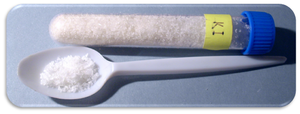
\includegraphics[scale=0.4]{KI.png}
\captionof{figure}{Kaliumjodid, \ch{KI}}
\label{fig6}
}





\vfill\null
\clearpage
\columnbreak
\newpage










                                     
                                     



